\chapter{Arbres et loi de Bernoulli}

\section{Représentation par un arbre pondéré}

\subsection{Modélisation}

\begin{methode}[Construire et utiliser un arbre]
	Un arbre pondéré permet de visualiser les probabilités conditionnelles.
	\begin{itemize}
		\item Le 1\textsuperscript{er} niveau donne les probabilités simples : $\p{A}$ et $\p{\bar{A}}$.
		\item Le 2\textsuperscript{e} niveau donne les probabilités conditionnelles : $\pc{A}{B}$, $\pc{A}{\bar{B}}$, etc.
	\end{itemize}

	\begin{center}
		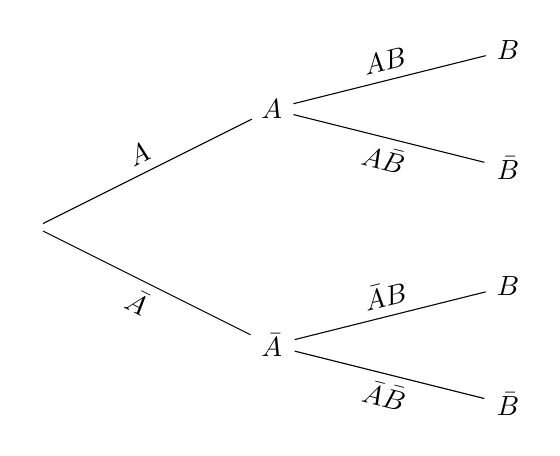
\begin{tikzpicture}[xscale=1, yscale=1]
			\tikzstyle{noeud} = [circle, inner sep=2pt]
			\tikzstyle{feuille} = [noeud]
			\node[noeud] (R) at (0,0) {};
			\node[noeud] (A) at (3,1.5) {$A$};
			\node[noeud] (Ab) at (3,-1.5) {$\bar{A}$};
			\node[feuille] (AB) at (6,2.25) {$B$};
			\node[feuille] (ABb) at (6,0.75) {$\bar{B}$};
			\node[feuille] (AbB) at (6,-0.75) {$B$};
			\node[feuille] (AbBb) at (6,-2.25) {$\bar{B}$};
			\draw (R) -- (A) node[sloped, midway, above] {$\p{A}$};
			\draw (R) -- (Ab) node[sloped, midway, below] {$\p{\bar{A}}$};
			\draw (A) -- (AB) node[sloped, midway, above] {$\pc{A}{B}$};
			\draw (A) -- (ABb) node[sloped, midway, below] {$\pc{A}{\bar{B}}$};
			\draw (Ab) -- (AbB) node[sloped, midway, above] {$\pc{\bar{A}}{B}$};
			\draw (Ab) -- (AbBb) node[sloped, midway, below] {$\pc{\bar{A}}{\bar{B}}$};
		\end{tikzpicture}
	\end{center}
\end{methode}

\begin{ex}
	\nline
	\begin{wrapstuff}[r]
		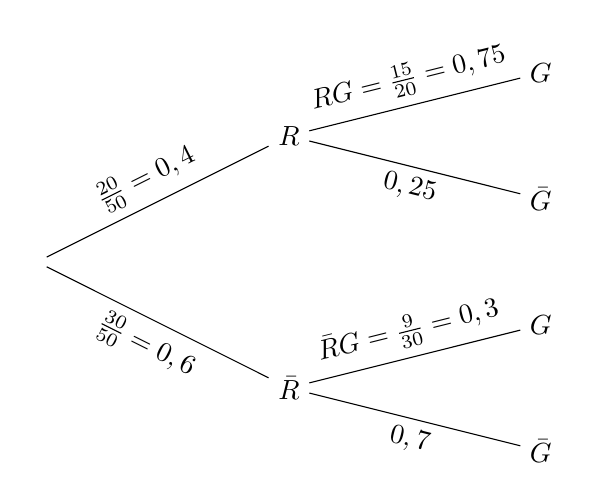
\begin{tikzpicture}[xscale=1.6, yscale=1.6]
			\node (R0) at (0,0) {};
			\node (A) at (2,1) {$R$};
			\node (B) at (2,-1) {$\bar{R}$};
			\node (AC) at (4,1.5) {$G$};
			\node (AD) at (4,0.5) {$\bar{G}$};
			\node (BC) at (4,-0.5) {$G$};
			\node (BD) at (4,-1.5) {$\bar{G}$};
			\draw (R0) -- (A) node[sloped, midway, above] {$\frac{20}{50}=0,4$};
			\draw (R0) -- (B) node[sloped, midway, below] {$\frac{30}{50}=0,6$};
			\draw (A) -- (AC) node[sloped, midway, above] {$\pc{R}{G}=\frac{15}{20}=0,75$};
			\draw (A) -- (AD) node[sloped, midway, below] {$0,25$};
			\draw (B) -- (BC) node[sloped, midway, above] {$\pc{\bar{R}}{G}=\frac{9}{30}=0,3$};
			\draw (B) -- (BD) node[sloped, midway, below] {$0,7$};
		\end{tikzpicture}
	\end{wrapstuff}

	Un sac contient $50$ boules, dont $20$ boules \textbf{rouges} et $30$ boules \textbf{noires}, marquées soit \og Gagné \fg{} soit \og Perdu \fg{}.

	\begin{itemize}
		\item Sur $15$ rouges, il est marqué Gagné.
		\item Sur $9$ noires, il est marqué Gagné.
	\end{itemize}

	Soient les événements :

	\begin{itemize}
		\item $R$ : \og On tire une boule rouge \fg{}
		\item $G$ : \og On tire une boule marquée Gagné \fg{}
	\end{itemize}

	\rule{0mm}{20mm}
\end{ex}

\begin{rem}
	On peut également modéliser cette situation à l'aide d'un tableau à double entrée :

	\begin{center}
		\rnc{\arraystretch}{1.3}
		\begin{tabular}{|l|c|c|c|}
			\hline
			~                     & \ccg Gagné : $G$ & \ccg Perdu : $\bar{G}$ & \ccg \textbf{Total} \\ \hline
			\ccg Rouge : $R$      & $15$             & $5$                    & $20$                \\ \hline
			\ccg Noir : $\bar{R}$ & $9$              & $21$                   & $30$                \\ \hline
			\ccg \textbf{Total}   & $24$             & $26$                   & $50$                \\ \hline
		\end{tabular}
	\end{center}
\end{rem}

\newpage

\subsection{Propriétés}

\begin{prop}[Règle \no 1]
	\nline
	\begin{wrapstuff}[r]
		\begin{tikzpicture}[>=Stealth,x=6mm,y=6mm]
			\draw[thick] (-1.5, 0) -- (1.5, 2.0);
			\draw[thick] (-1.5, 0) -- (1.5, -2.0);
			\node[circle, draw=blue, fill=gray!40, minimum size=5mm] (C1) at (0, 2.3) {};
			\node[font=\large\bfseries] (Plus) at (0, 0) {+};
			\node[circle, draw=blue, fill=gray!40, minimum size=5mm] (C2) at (0, -2.3) {};
			\node[font=\large\bfseries] (Eq) at (0, -4.5) {= 1};
			\draw[->, blue,thick] (C1.315) to[out=-45, in=45] (Plus.45);
			\draw[->, blue,thick] (Plus.315) to[out=-45, in=45] (C2.45);
			\draw[->, blue,thick] (C2.315) to[out=-45, in=45] (Eq.45);
		\end{tikzpicture}
	\end{wrapstuff}
	La somme des probabilités des branches issues d'un même noeud est égale à 1.

	\rule{0mm}{40mm}
\end{prop}

\begin{ex}
	$\p{R} + \p{\bar{R}} = 1 \implies\ \text{\og Soit on tire une boule rouge, soit une noire \fg{}}$
\end{ex}

\begin{prop}[Règle \no 2]
	\nline
	\begin{wrapstuff}[r]
		\begin{tikzpicture}[>=Stealth, x=6mm, y=6mm]
			\tikzstyle{noeud} = [circle, inner sep=2pt]
			\tikzstyle{poids} = [circle, draw=blue, fill=gray!40, minimum size=5mm]
			\node[noeud] (Racine) at (0,0) {};
			\node[noeud] (R) at (3,2) {$R$};
			\node[noeud] (Rb) at (3,-2) {$\bar{R}$};
			\node[noeud] (G) at (6,3.5) {$G$};
			\node[noeud] (Gb) at (6,0.5) {$\bar{G}$};
			\draw[ultra thick] (Racine) -- (R);
			\draw[ultra thick] (Racine) -- (Rb);
			\draw[ultra thick] (R) -- (G);
			\draw[ultra thick] (R) -- (Gb);
			\node[poids] (C1) at (1.2, 1.7) {};
			\node[font=\large\bfseries] (Mult) at (1.8, 3.3) {$\times$};
			\node[poids] (C2) at (4.0, 3.3) {};
			\node[font=\large] (Res) at (8.5, 4.2) {$=\p{R \cap G}$};
			\draw[->, blue, thick] (C1.80) to[out=60, in=180] (C2.180);
			\draw[->, blue, thick] (C2.55) to[out=35, in=180] (Res.180);
		\end{tikzpicture}
	\end{wrapstuff}
	La probabilité d'une \og feuille \fg{} (extrémité d'un chemin) est égale au \textbf{produit} des probabilités du chemin aboutissant à cette feuille.

	\rule{0mm}{35mm}
\end{prop}

\begin{ex}
	On considère la feuille $R \cap G$ :
	\[
		\p{R \cap G} = \p{R} \times \pc{R}{G} = 0,4 \times 0,75 = 0,3
	\]
\end{ex}

\begin{prop}[Règle \no 3 : "Probabilités totales"]
	La probabilité d'un événement associé à plusieurs \og feuilles \fg{} est égale à la \textbf{somme} des probabilités de chacune de ces \og feuilles \fg{}.
	\begin{center}
		\begin{tikzpicture}[>=Stealth, x=6mm, y=6mm]
			\tikzstyle{poids} = [circle, draw=blue, fill=gray!40, minimum size=5mm]
			\node (Racine) at (0,0) {};
			\node (R) at (3, 2.5) {$R$};
			\node (Rb) at (3, -2.5) {$\bar{R}$};
			\draw[ultra thick] (Racine) -- (R);
			\draw[ultra thick] (Racine) -- (Rb);
			\node (RG) at (6, 4) {$G$};
			\node (RGb) at (6, 1) {$\bar{G}$};
			\draw[ultra thick] (R) -- (RG);
			\draw[ultra thick] (R) -- (RGb);
			\node (RbG) at (6, -1) {$G$};
			\node (RbGb) at (6, -4) {$\bar{G}$};
			\draw[ultra thick] (Rb) -- (RbG);
			\draw[ultra thick] (Rb) -- (RbGb);
			\node[poids] (C1) at (1.2, 2.0) {};
			\node[font=\large\bfseries] (Mult1) at (1.7, 3.8) {$\times$};
			\node[poids] (C2) at (4.2, 3.9) {};
			\node[font=\large] (Res1) at (9.5, 4.2) {$= \p{R \cap G}$};
			\draw[->, blue, thick] (C1.80) to[out=60, in=180] (C2.180);
			\draw[->, blue, thick] (C2.35) to[out=35, in=160] (Res1.150);
			\node[poids] (C3) at (1.2, -2.0) {};
			\node[font=\large\bfseries] (Mult2) at (2.5, -0.1) {$\times$};
			\node[poids] (C4) at (4.5, -0.9) {};
			\node[font=\large] (Res2) at (9.5, -1.2) {$= \p{\bar{R} \cap G}$};
			\draw[->, blue, thick] (C3.70) to[out=60, in=160] (C4.150);
			\draw[->, blue, thick] (C4.55) to[out=35, in=160] (Res2.150);
			\node[font=\large] (Formule) at (16.5, 1.5) {$\p{G} = \p{R \cap G} + \p{\bar{R} \cap G}$};
			\node[font=\large] (Formule2) at (18.5, 1) {};
			\draw[->, blue, thick] (Res1.5) to[out=0, in=100] (Formule.100);
			\draw[->, blue, thick] (Res2.325) to[out=-40, in=-110] (Formule2.270);
		\end{tikzpicture}
	\end{center}
\end{prop}

\begin{ex}
	L'événement $G$ (\og On tire une boule marquée Gagné \fg{}) est associé aux feuilles $R \cap G$ et $\bar{R} \cap G$.
	\[
		\begin{array}{rcl}
			\p{G} & = & \p{R \cap G} + \p{\bar{R} \cap G} \\
			      & = & 0,3 + (0,6 \times 0,3)            \\
			      & = & 0,3 + 0,18 \qquad = 0,48
		\end{array}
	\]
\end{ex}

\begin{methode}[Calculer la probabilité d'un événement associé à plusieurs feuilles]
	\nline
	\begin{wrapstuff}[r]
		\begin{tikzpicture}[xscale=1.2, yscale=1.2]
			\node (R0) at (0,0) {};
			\node (F) at (2,1.1) {$F$};
			\node (G) at (2,-1.1) {$\bar{F}$};
			\node (FC) at (4,0.6) {$\bar{L}$};
			\node (FL) at (4,1.6) {$L$};
			\node (GC) at (4,-1.6) {$\bar{L}$};
			\node (GL) at (4,-0.6) {$L$};
			\draw (R0) -- (F) node[midway, sloped, above] {$0,65$};
			\draw (R0) -- (G) node[midway, sloped, below] {$0,35$};
			\draw (F) -- (FC) node[midway, sloped, below] {$\dfrac{1}{3}$};
			\draw (F) -- (FL) node[midway, sloped, above] {\color{rouge}$\dfrac{2}{3}$};
			\draw (G) -- (GC) node[midway, sloped, below] {$\dfrac{4}{5}$};
			\draw (G) -- (GL) node[midway, sloped, above] {\color{rouge}$\dfrac{1}{5}$};
		\end{tikzpicture}

	\end{wrapstuff}

	Dans une classe, il y a $65\%$ de filles.

	Un tiers des filles portent les cheveux courts, ainsi que $4$ garçons sur $5$.

	On choisit un élève au hasard.

	\begin{itemize}
		\item $F$ : \og l'élève choisi est une fille \fg{}
		\item $L$ : \og l'élève choisi a les cheveux longs \fg{}
	\end{itemize}

	Calculons $\p{L}$ :

	\begin{itemize}
		\item $\p{F \cap L} = \p{F} \times \pc{F}{L} = 0,65 \times \dfrac{2}{3} \implies$ \og Filles aux cheveux longs \fg{}
		\item $\p{\bar{F} \cap L} = \p{\bar{F}} \times \pc{\bar{F}}{L} = 0,35 \times \dfrac{1}{5} \implies$ \og Garçons aux cheveux longs \fg{}
	\end{itemize}

	D'après la formule des probabilités totales :
	\[
		\def\arraystretch{1.8}
		\begin{array}{rccll}
			\p{L} & = & \p{F \cap L}               & + & \p{\bar{F} \cap L}                                   \\
			      & = & 0{,}65 \times \dfrac{2}{3} & + & 0{,}35 \times \dfrac{1}{5} \qquad = \dfrac{151}{300}
		\end{array}
	\]
\end{methode}

\begin{methode}[Modéliser, compléter et calculer avec un arbre de probabilités]
	Dans une entreprise de fabrication de composants électroniques, deux chaînes de production approvisionnent le stock :
	\begin{itemize}
		\item La ligne $A$ produit $60\,\%$ des composants.
		\item La ligne $B$ produit le reste des composants.
	\end{itemize}

	Des tests de contrôle qualité révèlent que :
	\begin{itemize}
		\item $5\,\%$ des composants produits par la ligne $A$ présentent un défaut.
		\item $2\,\%$ des composants produits par la ligne $B$ présentent un défaut.
	\end{itemize}

	On prélève un composant au hasard dans le stock. On note les événements :
	\begin{itemize}
		\item $A$ : \og Le composant provient de la ligne $A$ \fg{} ;
		\item $B$ : \og Le composant provient de la ligne $B$ \fg{} ($\bar{A}$) ;
		\item $D$ : \og Le composant présente un défaut \fg{}.
	\end{itemize}

	\medskip

	Dans un exercice type, les questions suivent généralement une démarche progressive :
	\begin{itemize}
		\item \textbf{Étape 1 : Identifier les données de l'énoncé}
		      \begin{itemize}
			      \item Probabilités du 1\textsuperscript{er} niveau : $\p{A} = 0{,}60$ donc $\p{B} = \p{\bar{A}} = 1 - 0{,}60 = 0{,}40$ (\textit{Règle \no 1}).
			      \item Probabilités conditionnelles (2\textsuperscript{e} niveau) :
			            \begin{itemize}
				            \item Sachant $A$ : $\pc{A}{D} = 0{,}05$ donc $\pc{A}{\bar{D}} = 1 - 0{,}05 = 0{,}95$ (\textit{Règle \no 1}).
				            \item Sachant $B$ : $\pc{B}{D} = 0{,}02$ donc $\pc{B}{\bar{D}} = 1 - 0{,}02 = 0{,}98$ (\textit{Règle \no 1}).
			            \end{itemize}
		      \end{itemize}

		\item \textbf{Étape 2 : Construire et compléter l'arbre pondéré}
		      \begin{center}
			      \begin{tikzpicture}[x=15mm, >=Stealth]
				      \node (R) at (0,0) {};
				      \node (A) at (2.5,1.25) {$A$};
				      \node (B) at (2.5,-1.25) {$B$};
				      \node (AD) at (5,2) {$D$};
				      \node (ADb) at (5,0.75) {$\bar{D}$};
				      \node (BD) at (5,-0.75) {$D$};
				      \node (BDb) at (5,-2) {$\bar{D}$};
				      \draw[->, thick] (R) -- (A) node[sloped, midway, above] {$0{,}60$};
				      \draw[->, thick] (R) -- (B) node[sloped, midway, below,red] {$0{,}40$};
				      \draw[->, thick] (A) -- (AD) node[sloped, midway, above] {$0{,}05$};
				      \draw[->, thick] (A) -- (ADb) node[sloped, midway, below,red] {$0{,}95$};
				      \draw[->, thick] (B) -- (BD) node[sloped, midway, above] {$0{,}02$};
				      \draw[->, thick] (B) -- (BDb) node[sloped, midway, below,red] {$0{,}98$};
				      \node[vert, anchor=west] at (5.5,2)     {$\Rarr\p{A \cap D} = 0{,}60 \times 0{,}05 = 0{,}030$};
				      \node[vert, anchor=west] at (5.5,0.75)  {$\Rarr\p{A \cap \bar{D}} = 0{,}60 \times 0{,}95 = 0{,}570$};
				      \node[vert, anchor=west] at (5.5,-0.75) {$\Rarr\p{B \cap D} = 0{,}40 \times 0{,}02 = 0{,}008$};
				      \node[vert, anchor=west] at (5.5,-2)    {$\Rarr\p{B \cap \bar{D}} = 0{,}40 \times 0{,}98 = 0{,}392$};
			      \end{tikzpicture}
		      \end{center}

		\item \textbf{Étape 3 : Calculer des probabilités d'intersections (\textit{Règle \no 2})}
		      \begin{itemize}
			      \item Probabilité que le composant vienne de $A$ \textbf{et} soit défectueux :
			            \[
				            \p{A \cap D} = \p{A} \times \pc{A}{D} = 0{,}60 \times 0{,}05 = 0{,}03
			            \]
			      \item Probabilité que le composant vienne de $B$ \textbf{et} soit défectueux :
			            \[
				            \p{B \cap D} = \p{B} \times \pc{B}{D} = 0{,}40 \times 0{,}02 = 0{,}008
			            \]
		      \end{itemize}

		\item \textbf{Étape 4 : Calculer une probabilité totale $\p{D}$ (\textit{Règle \no 3})}

		      D'après la formule des probabilités totales :
		      \[
			      \def\arraystretch{1.7}
			      \begin{array}{rccccl}
				      \p{D} & = & \p{A \cap D} & + & \p{B \cap D} &           \\
				            & = & 0{,}03       & + & 0{,}008      & = 0{,}038
			      \end{array}
		      \]

		      La probabilité qu'un composant prélevé au hasard soit défectueux est donc égale à $3{,}8\,\%$.
	\end{itemize}
\end{methode}

\section{Expérience aléatoire à deux épreuves et épreuve de Bernoulli}

\subsection{Indépendance de deux événements}

\begin{defin}
	Deux expériences sont dites \textbf{indépendantes} si le résultat de l'une n'a aucune influence sur le résultat de l'autre.
\end{defin}

\begin{methode}[Calcul d'une probabilité associée à une expérience aléatoire à 2 épreuves]
	\nline
	\begin{wrapstuff}
		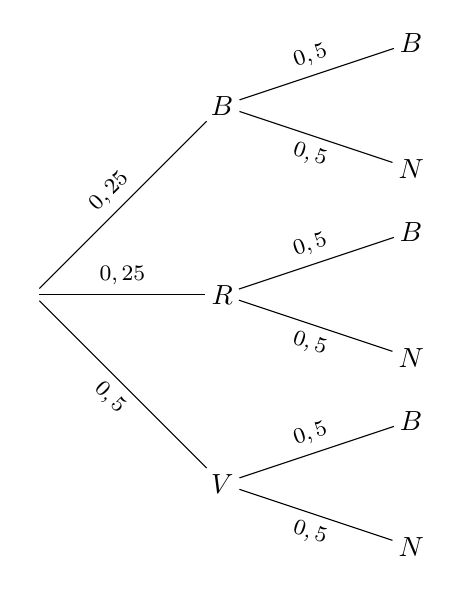
\begin{tikzpicture}[x=8mm, y=8mm]
			\tikzstyle{noeud} = [inner sep=2pt]
			\node[noeud] (R) at (0,0) {};
			\node[noeud] (B) at (3, 3) {$B$};
			\node[noeud] (Red) at (3, 0) {$R$};
			\node[noeud] (V) at (3, -3) {$V$};
			\node[noeud] (BB) at (6, 4) {$B$};
			\node[noeud] (BN) at (6, 2) {$N$};
			\node[noeud] (RB) at (6, 1) {$B$};
			\node[noeud] (RN) at (6, -1) {$N$};
			\node[noeud] (VB) at (6, -2) {$B$};
			\node[noeud] (VN) at (6, -4) {$N$};
			\draw (R) -- (B) node[sloped, midway, above,font=\footnotesize] {$0,25$};
			\draw (R) -- (Red) node[sloped, midway, above,font=\footnotesize] {$0,25$};
			\draw (R) -- (V) node[sloped, midway, below,font=\footnotesize] {$0,5$};
			\draw (B) -- (BB) node[sloped, midway, above,font=\footnotesize] {$0,5$};
			\draw (B) -- (BN) node[sloped, midway, below,font=\footnotesize] {$0,5$};
			\draw (Red) -- (RB) node[sloped, midway, above,font=\footnotesize] {$0,5$};
			\draw (Red) -- (RN) node[sloped, midway, below,font=\footnotesize] {$0,5$};
			\draw (V) -- (VB) node[sloped, midway, above,font=\footnotesize] {$0,5$};
			\draw (V) -- (VN) node[sloped, midway, below,font=\footnotesize] {$0,5$};
		\end{tikzpicture}
	\end{wrapstuff}
	Léa tente l'expérience suivante avec ses vêtements :

	Elle dépose dans un panier $4$ chemisiers indiscernables au toucher :

	\begin{itemize}
		\item $1$ blanc
		\item $1$ rouge
		\item $2$ verts
	\end{itemize}

	Dans un autre panier, elle y dépose $2$ jupes indiscernables au toucher :

	\begin{itemize}
		\item $1$ blanche
		\item $1$ noire
	\end{itemize}

	Elle tire au hasard, un chemisier du 1\up{er} panier et une jupe du 2\up{ème} panier.

	Il s'agit de deux tirages successifs effectués dans des paniers distincts : le résultat du premier tirage n'impacte pas les probabilités du second.

	Les deux expériences sont donc \textbf{indépendantes}.

	\rule{0mm}{5mm}
\end{methode}

\begin{rem}
	Sur l'arbre de probabilités, cela se traduit par le fait que les sous-arbres du second niveau (issus de B, R et V) sont rigoureusement \textbf{identiques}.
\end{rem}

\newpage

\subsection{Épreuve de Bernoulli}

\begin{defin}{}
	Une \textbf{épreuve de Bernoulli} est une expérience aléatoire à \textbf{deux issues} que l'on nomme traditionnellement \og \textbf{succès} \fg{} (noté $S$) et \og \textbf{échec} \fg{} (noté $\bar{S}$).

	La probabilité du succès est notée $p$ et la probabilité de l'échec est alors égale à $\pa{1 - p}$.

	\begin{center}
		\begin{tikzpicture}[x=6mm, y=6mm, >=Stealth]
			\tikzstyle{noeud} = [inner sep=2pt]
			\node[noeud] (R) at (0,0) {};
			\node[noeud] (S) at (3, 1.5) {Succès};
			\node[noeud] (E) at (3, -1.5) {Échec};
			\draw[thick, ->] (R) -- (S) node[sloped, midway, above] {$p$};
			\draw[thick, ->] (R) -- (E) node[sloped, midway, below] {$1-p$};
		\end{tikzpicture}
	\end{center}
\end{defin}

\begin{rem}
	\nline
	\begin{itemize}
		\item Au succès, on peut associer le nombre $1$
		\item À l'échec, on peut associer le nombre $0$
	\end{itemize}
\end{rem}

\begin{ex}
	\nline
	\begin{itemize}
		\item Le jeu du pile ou face :

		      On considère comme \textbf{succès} "obtenir pile" et comme \textbf{échec} "obtenir face"
		\item Un lancer un dé à six faces :

		      On considère comme \textbf{succès} "obtenir un $\epsdice{1}$" et comme \textbf{échec} "ne pas obtenir un $\epsdice{1}$"
	\end{itemize}
\end{ex}

\begin{defin}
	\nline
	\begin{wrapstuff}[r]
		\begin{tikzpicture}[x=6mm, y=6mm, >=Stealth]
			\tikzstyle{noeud} = [inner sep=2pt]
			\node[noeud] (R) at (0,0) {};
			\node[noeud] (S) at (3, 1.5) {Succès};
			\node[noeud] (E) at (3, -1.5) {Échec};
			\draw[thick, ->] (R) -- (S) node[sloped, midway, above] {$p$};
			\draw[thick, ->] (R) -- (E) node[sloped, midway, below] {$1-p$};
		\end{tikzpicture}
	\end{wrapstuff}
	Soit une épreuve de Bernoulli.

	On appelle $X$ la variable aléatoire qui prend :

	\begin{itemize}
		\item \ldots la valeur $1$ en cas de \textbf{succès}
		\item \ldots et la valeur $0$ en cas d'\textbf{échec}.
	\end{itemize}

	La loi de probabilité de $X$ est appelée \textbf{loi de Bernoulli} de paramètre $p$, où $p$ est la probabilité du succès.

	On peut résumer cette loi dans le tableau suivant :

	\begin{center}
		\renewcommand{\arraystretch}{1.5}
		\begin{tabular}{|c|c|c|} \hline
			\ccg $x_i$      & $1$ & $0$        \\ \hline
			\ccg $P(X=x_i)$ & $p$ & $\pa{1-p}$ \\ \hline
		\end{tabular}
	\end{center}
\end{defin}

\begin{ex}
	\nline
	\begin{itemize}
		\item Le jeu du pile ou face :

		      $S$=\og Faire pile\fg{} $\quad\rarr p=\dfrac{1}{2}=0.5$
		      \begin{center}
			      \rnc{\arraystretch}{1.3}
			      \begin{tabular}{|c|c|c|} \hline
				      \ccg $x_i$       & $1$   & $0$   \\ \hline
				      \ccg $\p{X=x_i}$ & $0.5$ & $0.5$ \\ \hline
			      \end{tabular}
		      \end{center}

		\item Lancer un dé

		      $S$=\og Faire \epsdice{1}\fg{} $\quad\rarr p=\dfrac{1}{6}$
		      \begin{center}
			      \rnc{\arraystretch}{1.5}
			      \begin{tabular}{|c|c|c|} \hline
				      \ccg $x_i$       & $1$           & $0$           \\ \hline
				      \ccg $\p{X=x_i}$ & $\frac{1}{6}$ & $\frac{5}{6}$ \\ \hline
			      \end{tabular}
		      \end{center}
	\end{itemize}

\end{ex}

\begin{methode}[Reconnaître une situation modélisée par une loi de Bernoulli]
	\nline
	\begin{wrapstuff}[r]
		\begin{tikzpicture}[x=8mm, y=8mm, >=Stealth]
			\tikzstyle{noeud} = [inner sep=2pt]
			\node[noeud] (R) at (0,0) {};
			\node[noeud] (S) at (3, 1.5) {$S$};
			\node[noeud] (E) at (3, -1.5) {$\bar{S}$};
			\draw[thick, ->] (R) -- (S) node[sloped, midway, above] {$0{,}8$};
			\draw[thick, ->] (R) -- (E) node[sloped, midway, below] {$0{,}2$};
		\end{tikzpicture}
	\end{wrapstuff}
	Après la correction d'un contrôle, le professeur compte que $24$ élèves ont obtenu une note $\ge 10$ et $6$ ne l'ont pas obtenue.

	Le professeur choisit une copie au hasard.

	Cette expérience aléatoire possède $2$ issues.

	\begin{itemize}
		\item Succès $S$ : \og la copie indique une note $\ge 10$ \fg{} ;
		\item Échec $\bar{S}$ : \og la copie indique une note $< 10$ \fg{}.
	\end{itemize}

	La probabilité de l'issue "la copie indique une note $\ge 10$" est égale à :
	\[
		p=\frac{24}{30}=\frac{4}{5}=0{,}8
	\]

	La situation est donc modélisée par une loi de \textbf{Bernoulli} de paramètre $p=\dfrac{4}{5}=0{,}8$.
\end{methode}

\subsection{Espérance}

\begin{prop}
	Soit $X$ une variable aléatoire qui suit la loi de \textbf{Bernoulli} de paramètre $p$.

	Alors l'espérance mathématique de $X$ est :
	\[
		{E(X)=p}
	\]
\end{prop}

\begin{ex}
	On considère une urne contenant $50$ boules au total :

	\begin{itemize}
		\item $27$ boules blanches
		\item $23$ boules noires
	\end{itemize}

	On tire une boule au hasard dans l'urne. On s'intéresse à l'événement \og obtenir une boule noire \fg{}.

	Soit $X$ la variable aléatoire qui prend la valeur :

	\begin{itemize}
		\item $1$ si la boule tirée est noire (succès)
		\item $0$ si elle est blanche (échec)
	\end{itemize}

	$X$ suit la loi de Bernoulli de paramètre $p = \frac{23}{50} = 0{,}46$.

	L'espérance mathématique de $X$ est alors :
	\[
		E(X) = p = 0{,}46
	\]

	\textbf{Interprétation :}

	Cela signifie qu'en répétant ce tirage un grand nombre de fois dans les mêmes conditions, on obtiendra en moyenne \textbf{$0{,}46$ boule noire par tirage} (soit $46\,\%$ de boules noires tirées).
\end{ex}

\begin{demo}
	Soit $X$ une variable aléatoire qui suit la loi de \textbf{Bernoulli} de paramètre $p$.

	On a :

	\begin{center}
		\rnc{\arraystretch}{1.3}
		\begin{tabular}{|c|c|c|} \hline
			\ccg $x_i$       & $1$ & $0$        \\ \hline
			\ccg $\p{X=x_i}$ & $p$ & $\pa{1-p}$ \\ \hline
		\end{tabular}
	\end{center}

	Donc :
	\[
		\begin{array}{rccccl}
			E(X) & = & p_1\times x_1 & + & p_2\times x_2   &     \\
			     & = & 1\times p     & + & 0\times (1 - p) & = p
		\end{array}
	\]
\end{demo}

\subsection{Répétitions d'épreuves de Bernoulli}

\begin{defin}
	Plusieurs expériences sont \textbf{identiques et indépendantes} si :

	\begin{itemize}
		\item \ldots elles ont les mêmes issues,
		\item \ldots chaque issue possède la même probabilité.
	\end{itemize}
\end{defin}

\begin{ex}
	\nline
	\begin{wrapstuff}[r]
		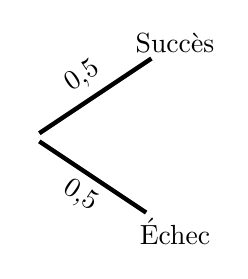
\begin{tikzpicture}[x=6mm, y=6mm]
			\tikzstyle{noeud} = [inner sep=2pt]
			\node[noeud] (R) at (0,0) {};
			\node[noeud] (S) at (3, 2) {Succès};
			\node[noeud] (E) at (3, -2) {Échec};
			\draw[ultra thick] (R) -- (S) node[sloped, midway, above] {$0{,}5$};
			\draw[ultra thick] (R) -- (E) node[sloped, midway, below] {$0{,}5$};
		\end{tikzpicture}
	\end{wrapstuff}

	On lance $20$ fois de suite une pièce de monnaie.

	On considère :

	\begin{itemize}
		\item Succès : \og obtenir Pile \fg{} ;
		\item Échec : \og obtenir Face \fg{}.
	\end{itemize}

	Ces expériences de \textbf{Bernoulli} sont \textbf{identiques et indépendantes}.

	On dit que $p=0,5$ est le \textbf{paramètre} de l'épreuve de \textbf{Bernoulli} répétée $20$ fois.
\end{ex}

\begin{ex}
	On lance $5$ fois un dé à six faces et on note à chaque fois le résultat.

	À chaque lancer, on considère :

	\begin{itemize}
		\item Succès : \og obtenir un \epsdice{6} \fg{} ;
		\item Échec : \og ne pas obtenir un \epsdice{6} \fg{}.
	\end{itemize}

	On répète ainsi $5$ fois de suite la même expérience de \textbf{Bernoulli} (lancer un dé) et les expériences sont \textbf{indépendantes} l'une de l'autre : un lancer n'influence pas le résultat d'un autre lancer.

	On dit que $p=\dfrac{1}{6}$ est le \textbf{paramètre} de l'épreuve de \textbf{Bernoulli} répétée \textbf{$5$ fois}.
\end{ex}

\begin{methode}[Calculer une probabilité associée à une épreuve de Bernoulli]
	On considère l'expérience suivante :

	Une urne contient $3$ boules blanches et $2$ boules rouges.

	On tire au hasard une boule et \textbf{on la remet dans l'urne}.

	On répète l'expérience $2$ fois de suite.

	\begin{itemize}
		\item Représenter l'ensemble des issues de ces expériences dans un arbre.
		\item Déterminer les probabilités suivantes :
		      \begin{enumerate}
			      \item On tire deux boules blanches
			      \item On tire une boule blanche et une boule rouge
			      \item On tire au moins une boule blanche
		      \end{enumerate}
	\end{itemize}

	\begin{correction}
		On note :

		\begin{itemize}
			\item $A$ l'issue "On tire une boule blanche" $\quad\rarr \p{A}=\dfrac{3}{5}=0,6$
			\item $\bar{A}$ l'issue contraire "On tire une boule rouge" $\quad\rarr \p{\bar{A}}=\dfrac{2}{5}=0,4$
		\end{itemize}

		\begin{center}
			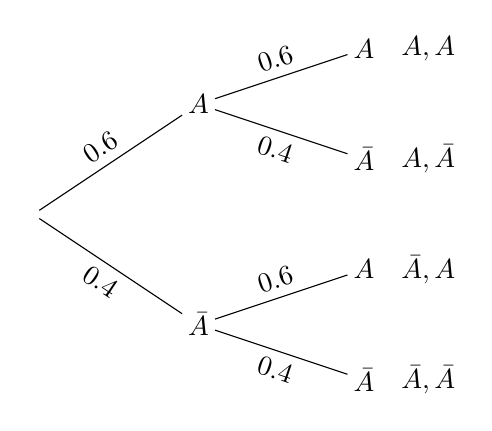
\begin{tikzpicture}[x=7mm, y=7mm]
				\tikzstyle{noeud} = [inner sep=2pt]
				\node[noeud] (Racine) at (0,0) {};
				\node[noeud] (B1) at (3, 2) {$A$};
				\node[noeud] (R1) at (3, -2) {$\bar{A}$};
				\node[noeud] (BB) at (6, 3) {$A$};
				\node[noeud] (BR) at (6, 1) {$\bar{A}$};
				\node[noeud] (RB) at (6, -1) {$A$};
				\node[noeud] (RR) at (6, -3) {$\bar{A}$};
				\node[anchor=west] at (6.5, 3) {$\pa{A, A}$};
				\node[anchor=west] at (6.5, 1) {$\pa{A, \bar{A}}$};
				\node[anchor=west] at (6.5, -1) {$\pa{\bar{A}, A}$};
				\node[anchor=west] at (6.5, -3) {$\pa{\bar{A}, \bar{A}}$};
				\draw (Racine) -- (B1) node[sloped, midway, above] {$0.6$};
				\draw (Racine) -- (R1) node[sloped, midway, below] {$0.4$};
				\draw (B1) -- (BB) node[sloped, midway, above] {$0.6$};
				\draw (B1) -- (BR) node[sloped, midway, below] {$0.4$};
				\draw (R1) -- (RB) node[sloped, midway, above] {$0.6$};
				\draw (R1) -- (RR) node[sloped, midway, below] {$0.4$};
			\end{tikzpicture}
		\end{center}

		\begin{enumerate}
			\item Obtenir deux boules blanches correspond à l'issue $\pa{A ;A}$ :
			      \[
				      P_1 = \p{AA} = 0,6 \times 0,6 = 0,36
			      \]
			\item Obtenir une blanche et une rouge correspond aux issues $\pa{ A ; \bar{A} }$ et $\pa{\bar{A} ;A}$
			      \[
				      \def\arraystretch{1.1}
				      \begin{array}{rccccr}
					      P_2 & = & \p{A\bar{A}}  & + & \p{\bar{A}A}  & ~          \\
					      ~   & = & 0,6\times 0,4 & + & 0,4\times 0,6 & ~          \\
					      ~   & = & 0,24          & + & 0,24          & \quad=0,48
				      \end{array}
			      \]

			\item Obtenir \textbf{au moins} une blanche correspond à $\pa{A;\bar{A}}$, $\pa{A;A}$ et $\pa{\bar{A} ;A}$
			      \[
				      \def\arraystretch{1.1}
				      \begin{array}{rccccccr}
					      P_3 & = & \p{A\bar{A}}  & + & \p{AA}        & + & \p{\bar{A}A}  & ~          \\
					      ~   & = & 0,6\times 0,4 & + & 0,6\times 0,6 & + & 0,4\times 0,6 & ~          \\
					      ~   & = & 0,24          & + & 0,36          & + & 0,24          & \quad=0,84
				      \end{array}
			      \]
		\end{enumerate}

		\textbf{Arbre de probabilité de la situation :}
		\begin{center}
			\begin{tikzpicture}[x=8mm, y=7mm, >=Stealth]
				\tikzstyle{noeud} = [inner sep=2pt]
				\node[noeud] (R) at (0,0) {};
				\node[noeud] (A1) at (4, 2.5) {$A$};
				\node[noeud] (A1bar) at (4, -2.5) {$\bar{A}$};
				\node[noeud] (A2_1) at (8, 3.5) {$A$};
				\node[noeud] (A2_2) at (8, 1.5) {$\bar{A}$};
				\node[noeud] (A2_3) at (8, -1.5) {$A$};
				\node[noeud] (A2_4) at (8, -3.5) {$\bar{A}$};
				\draw[thick, ->] (R) -- (A1) node[sloped, midway, above, blue] {$0{,}6$};
				\draw[thick, ->] (R) -- (A1bar) node[sloped, midway, below, blue] {$0{,}4$};
				\draw[thick, ->] (A1) -- (A2_1) node[sloped, midway, above, blue] {$0{,}6$};
				\draw[thick, ->] (A1) -- (A2_2) node[sloped, midway, below, blue] {$0{,}4$};
				\draw[thick, ->] (A1bar) -- (A2_3) node[sloped, midway, above, blue] {$0{,}6$};
				\draw[thick, ->] (A1bar) -- (A2_4) node[sloped, midway, below, blue] {$0{,}4$};
				\draw[->, dashed, vert, thick] (8.8, 3.5) -- (10.5, 3.5) node[right, vert] {$0{,}6 \times 0{,}6 = 0{,}36$};
				\draw[->, dashed, vert, thick] (8.8, 1.5) -- (10.5, 1.5) node[right, vert] {$0{,}6 \times 0{,}4 = 0{,}24$};
				\draw[->, dashed, vert, thick] (8.8, -1.5) -- (10.5, -1.5) node[right, vert] {$0{,}4 \times 0{,}6 = 0{,}24$};
				\draw[->, dashed, vert, thick] (8.8, -3.5) -- (10.5, -3.5) node[right, vert] {$0{,}4 \times 0{,}4 = 0{,}16$};
			\end{tikzpicture}
		\end{center}
	\end{correction}
\end{methode}
\begin{rem}
	Dans cette situation, on peut définir une variable aléatoire $X$ qui compte le nombre de boules blanches obtenues (c'est-à-dire le nombre de succès) au cours des $2$ tirages.

	La variable aléatoire $X$ peut prendre les valeurs $0$, $1$ ou $2$.

	\begin{itemize}
		\item $\p{X = 0} = \p{\bar{A}\bar{A}} = 0{,}4 \times 0{,}4 = 0{,}16$ ;
		\item $\p{X = 1} = \p{A\bar{A}} + \p{\bar{A}A} = 0{,}6 \times 0{,}4 + 0{,}4 \times 0{,}6 = 0{,}24 + 0{,}24 = 0{,}48$ ;
		\item $\p{X = 2} = \p{AA} = 0{,}6 \times 0{,}6 = 0{,}36$.
	\end{itemize}

	On peut alors établir la loi de probabilité de $X$ sous la forme d'un tableau :

	\begin{center}
		\renewcommand{\arraystretch}{1.5}
		\begin{tabular}{|c|c|c|c|} \hline
			\ccg $x_i$         & $0$      & $1$      & $2$      \\ \hline
			\ccg $\p{X = x_i}$ & $0{,}16$ & $0{,}48$ & $0{,}36$ \\ \hline
		\end{tabular}
	\end{center}

	On vérifie bien que la somme des probabilités est égale à $1$ :
	\[
		0{,}16 + 0{,}48 + 0{,}36 = 1
	\]

	La répétition de telles épreuves de Bernoulli identiques et indépendantes constitue ce que l'on appelle un \textbf{schéma de Bernoulli}, et la variable aléatoire $X$ qui compte le nombre de succès suit une loi bien spécifique appelée \textbf{loi binomiale}.
\end{rem}

